\documentclass[twocolumn]{article}
\setlength{\columnsep}{20pt}
%\usepackage{url}
%\usepackage{algorithmic}
\usepackage[a4paper]{geometry}
\usepackage{datetime}
\usepackage[font=small,labelfont=it]{caption}
\usepackage{graphicx}
% Use Times NR as font
\usepackage{lmodern}
\usepackage[T1]{fontenc}

\usepackage{float}

% Better tables
\usepackage{tabularx}
% to make beautiful tables
\usepackage{booktabs}

\usepackage{microtype}
\usepackage{amsmath}
\usepackage{subfigure}

% Letterspacing macros
\newcommand{\spacecaps}[1]{\textls[200]{\MakeUppercase{#1}}}
\newcommand{\spacesc}[1]{\textls[50]{\textsc{\MakeLowercase{#1}}}}

\title{\huge{\textbf{Study doc: regularisation experiment}}\\ \normalsize \Large{how does the regularisation factors effect the embedding space}}

\author{Fabian Gröger\\fabian.groeger@stud.hslu.ch}
\date{\today}

\begin{document}
\maketitle

\begin{abstract}
The experiment aims to show how the embedding space will change for different regularisation factors.
\end{abstract}

\section{Introduction}
The purpose of regularisation is that it prevents models from overfitting, by penalising high weights. The regularisation is calculated for all layers weights separately and is then added to the standard loss function, in this case, the triplet loss. The combined loss value is then used to calculate the gradients and update the weights of the model. There are a lot of different regularisation techniques, which successfully reduce the chance of overfitting. In this experiment, the \texttt{L2-Regularisation} is used and evaluated with different values. The parameter which will control the value of the \texttt{L2-Regularisation} is denoted as $\lambda$.

\section{Hyperparameters}
The hyperparameters used for this experiment are shown in table \ref{tab:Hyperparameters}. The experiment will be conducted using a state of the art ResNet18 architecture on the DCASE dataset. The hyperparameters in section \textit{Feature representation} as well as the sample rate are the default ones proposed by the organisers of the DCASE challenge within the baseline project. The regularisation factor $\lambda$ will be evaluated for three different values \texttt{[1.0, 0.1, 0.01]}.

\begin{table}[H]
    \centering
    \caption{Hyperparameters used for the experiment}
	\label{tab:Hyperparameters}
    \begin{tabular}{l|l}
        \toprule
        \textbf{Hyperparameter} & \textbf{value} \\ 
        \midrule[1pt]
        Dataset & DCASE \\
        \hline
        Model & ResNet18 \\ 
        \hline
        Epochs & 30-50 \\ 
        \hline
        Batch size & 128 \\ 
        \hline
        Optimizer & Adam \\ 
        \hline
        Learning rate & 1e-5 \\
        \hline
        Margin & 1.0 \\
        \hline
        L2 regularisation factor & \textbf{[1.0, 0.1, 0.01]} \\
        \hline
        Embedding dimension & 64 \\
        \hline
        Prefetch batches & Autotune (-1) \\ 
        \hline
        Random selection buffer & 64 \\ 
        \hline
        Shuffle dataset & True \\
        \hline
        Random seed & 1234 \\
        \midrule[1pt]
        \multicolumn{2}{l}{\textit{Multi threading}} \\
        \midrule[1pt]
        Number of generators & 16 \\ 
        \hline
        Number of parallel calls & 16 \\
        \midrule[1pt]
        \multicolumn{2}{l}{\textit{Audio sample}} \\
        \midrule[1pt]
        Sample rate & 16000 \\ 
        \hline
        Sample size & 10 \\
        \hline
        Sample tile size & 5 \\
        \hline
        Sample tile range & 5 \\
        \hline
        Convert to mono & True \\
        \midrule[1pt]
        \multicolumn{2}{l}{\textit{Feature representation}} \\
        \midrule[1pt]
        Feature extractor & LogMelExtractor \\ 
        \hline
        Frame length & 480 \\
        \hline
        Frame step & 160 \\
        \hline
        FFT size & 1024 \\
        \hline
        Number of Mel bins & 128 \\
        \hline
        Number of MFCC bins & 13 \\
        \bottomrule
    \end{tabular}
\end{table}

\begin{figure}[t]
\centering
    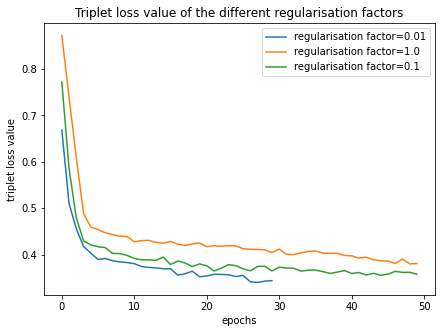
\includegraphics[width=\linewidth]{assets/triplet_loss.png}
    \caption{Plot of the triplet loss values of the different regularisation factors $\lambda$}
    \label{fig:plot-triplet-loss}
\end{figure}

\section{Results}
Comparing the effect of different regularisation factors on the embedding space is pretty hard, since comparing embedding spaces is not very straight forward and is a rather tricky task. This is mainly because of the fact, that to visualise the high dimensional embedding space in a way humans can perceive it, it has to be reduced to two or three dimensions. Therefore the original space can not be examined, and the visual representation is always an approximation of the space in a lower dimension. To still compare the embedding spaces and the effect of $\lambda$, a simple logistic classifier is trained on top of the resulting embedding spaces, which aims to show how well a simple classifier works with the embedding space. This will show how good the resulting embedding space is. The classifier is trained for 20 epochs with the same parameters as the embedding model (table \ref{tab:Hyperparameters}).

Figure \ref{fig:plot-triplet-loss} shows the difference between the triplet loss values of the embedding model when changing the regularisation factor. It shows that the model with $\lambda = 1.0$ has the highest triplet loss value, which is obvious, since the bigger the regularisation factor is, the longer the model optimises the weights to satisfy the constraint of having very small weights. The lower $\lambda$, the faster the model optimises the triplet loss value. $\lambda = 0.01$ has the lowest triplet loss value.

Figure \ref{fig:classifier-f1} shows the different F1 scores of the logistic classifier, which is trained on top of the embedding architecture. This provides an idea of how well the embedding space separates the classes and therefore gives a performance gain. The figure \ref{fig:classifier-f1} shows, that the regularisation factor $\lambda = 0.01$ has the highest F1 score. This result is significant since this particular embedding space was only trained for 30 epochs, unlike the other models, who are trained for 50. 

The figure \ref{fig:classifier-loss} shows the corresponding categorical cross-entropy loss values of the trained classifiers. It shows that the loss of $\lambda = 1.0$ converges before $\lambda = 0.1$ or $\lambda = 0.01$. The figure further shows, that the loss values of $\lambda = 0.1$ and $\lambda = 0.01$ are not converged and would benefit from a longer training.

\begin{figure}[t]
\centering
    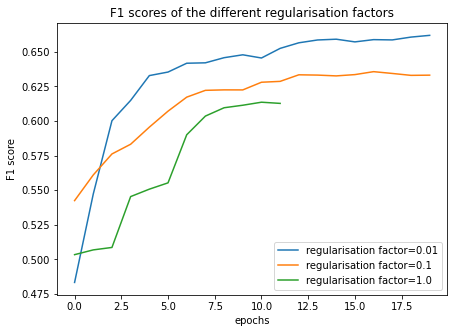
\includegraphics[width=\linewidth]{assets/classifier_f1.png}
    \caption{Line plot of the F1 score from the different classifiers trained on top of the resulting embedding spaces}
    \label{fig:classifier-f1}
\end{figure}

\begin{figure}[t]
\centering
    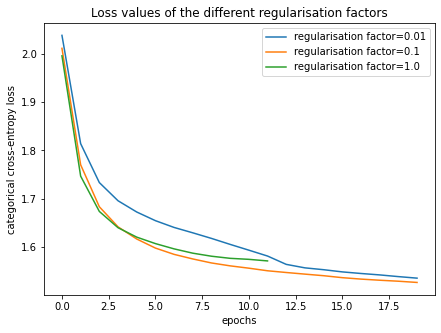
\includegraphics[width=\linewidth]{assets/classifier_loss.png}
    \caption{Line plot of the sparse categorical cross-entropy loss of the embedding size 16 and 64}
    \label{fig:classifier-loss}
\end{figure}

\section{Conclusion}
Figure \ref{fig:classifier-f1} shows that the highest regularisation factor $\lambda = 1.0$ can be omitted since it did not accomplish an equally good F1 score. This result is expectable since a high regularisation factor forces the embedding model to work with very small weights and can, therefore, lead to performance loss. 

The regularisation factor $\lambda = 0.1$ and $\lambda = 0.01$ only show very little difference in F1 performance as well as in triplet loss value. Never the less, the factor $\lambda = 0.01$ provides slightly better results than $\lambda = 0.1$. 

The triplet loss value and the loss value of the classifier of the regularisation factor $\lambda = 0.01$ is still decreasing at the end of the training, which indicates that the model can benefit from further training. Further training will increase the resulting embedding space and the F1 score of the classifier until it converges.

The figure \ref{fig:plot-triplet-loss} and \ref{fig:classifier-f1} further indicate one very important conclusion, that the value of the triplet loss is directly related to how well the classifier performs, which is further an indication how well the created embedding space works. Therefore the assumption is, that the lower the triplet loss value, the better the classifier performs and the better the embedding space is. 

The experiment shows that the regularisation factor $\lambda = 0.01$ gives the best results out of the three since it has an optimal triplet loss value, a high enough F1 score and the loss value still decreases after 20 epochs of training the classifier.

\section{Next steps}
The experiment showed that the regularisation factor $\lambda$ has an essential impact on the embedding space and should therefore not be chosen to be too big nor too small since this either leads to over- or underfitting. The optimal regularisation parameter $\lambda$ should be further examined in later and more extensive experiments with a lot more values for $\lambda$.

For the next experiments, the regularisation factor $\lambda = 0.01$ is chosen.

\end{document}